\documentclass{book}

\usepackage{ctex}
\usepackage{lipsum}
\usepackage{amsmath, amsthm, amssymb, amsfonts,mathrsfs}
\usepackage{thmtools}
\usepackage{graphicx}
\usepackage{setspace}
\usepackage{geometry}
\geometry{
  a4paper,
  top=25.4mm, bottom=25.4mm,
  left=20mm, right=20mm,
  headheight=2.17cm,
  headsep=4mm,
  footskip=12mm
}
\usepackage{float}
\usepackage{hyperref}
\usepackage[utf8]{inputenc}
\usepackage[english]{babel}
\usepackage{framed}
\usepackage[dvipsnames]{xcolor}
\usepackage{tikz-cd}
\usepackage[most]{tcolorbox}
\usepackage{ctex}
\usepackage{pifont}
\usepackage{framed}
\definecolor{shadecolor}{RGB}{241, 241, 255}
\newcounter{problemname}

\tcbuselibrary{theorems}
\tcbuselibrary{breakable}
\hypersetup{hidelinks,
	colorlinks=true,
	allcolors=black,
	pdfstartview=Fit,
	breaklinks=true
}

%定义颜色,可以根据需求自己修改
\definecolor{LightIndigo}{HTML}{E0FFFF}
\colorlet{LightGray}{White!90!Periwinkle}
\colorlet{LightOrange}{Orange!15}
\colorlet{LightGreen}{Green!15}
\colorlet{Lightblue}{Blue!15}
\colorlet{Lightpurple}{Purple!15}
\colorlet{LightRed}{Red!15}
\colorlet{LightYellow}{Yellow!15}
\colorlet{LightCyan}{Cyan!15}
%\colorlet{LightIndigo}{E0FFFF}

\newcommand{\HRule}[1]{\rule{\linewidth}{#1}}

\newtheorem{corollary}{Corollary}[section]
\newenvironment{solution}{{\noindent\it Solution.} }{\hfill $\square$\par}
\newenvironment{note}{\noindent\it Note.}{\par}

\declaretheoremstyle[name=Theorem,]{thmsty}
\declaretheorem[style=thmsty,numberwithin=section]{theorem}
\tcolorboxenvironment{theorem}{colback=LightGray,breakable,before upper app={\setlength{\parindent}{2em}}}

\declaretheoremstyle[name=Definition,]{thmsty}
\declaretheorem[style=thmsty,numberwithin=section]{definition}
\tcolorboxenvironment{definition}{colback=LightCyan,breakable,before upper app={\setlength{\parindent}{2em}}}

\declaretheoremstyle[name=Remark,]{thmsty}
\declaretheorem[style=thmsty,numberwithin=section]{remark}
\tcolorboxenvironment{remark}{colback=LightRed,breakable,before upper app={\setlength{\parindent}{2em}}}

\declaretheoremstyle[name=Lemma,]{thmsty}
\declaretheorem[style=thmsty,numberwithin=section]{lemma}
\tcolorboxenvironment{lemma}{colback=Lightblue,breakable,before upper app={\setlength{\parindent}{2em}}}

\declaretheoremstyle[name=Corollary,]{thmsty}
\declaretheorem[style=thmsty,numberwithin=section]{Corollary}
\tcolorboxenvironment{corollary}{colback=Lightpurple,breakable,before upper app={\setlength{\parindent}{2em}}}

\declaretheoremstyle[name=Proposition,]{prosty}
\declaretheorem[style=prosty,numberwithin=section]{proposition}
\tcolorboxenvironment{proposition}{colback=LightOrange,breakable,before upper app={\setlength{\parindent}{2em}}}

\declaretheoremstyle[name=Example,]{prosty}
\declaretheorem[style=prosty,numberwithin=section]{example}
\tcolorboxenvironment{example}{colback=LightGreen,breakable,before upper app={\setlength{\parindent}{2em}}}

\declaretheoremstyle[name=Exercise,]{prosty}
\declaretheorem[style=prosty,numberwithin=section]{exercise}
\tcolorboxenvironment{exercise}{colback=LightYellow,breakable,before upper app={\setlength{\parindent}{2em}}}

\setstretch{1.2}
\geometry{
    textheight=9in,
    textwidth=5.5in,
    top=1in,
    headheight=12pt,
    headsep=25pt,
    footskip=30pt
}
\usepackage{float}
\title{ \normalsize \textsc{Notes of Functional Analysis}
		\\ [2.0cm]
		\HRule{1.5pt} \\
		\LARGE \textbf{\uppercase{泛函分析笔记}
		\HRule{2.0pt} \\ [0.6cm] \LARGE{Jinhua Wu} \vspace*{10\baselineskip}}
		}
\date{}
\author{}
\begin{document}
\maketitle
\tableofcontents 
\newpage
\setcounter{page}{1}
\chapter{度量空间}
\begin{definition}
    设$X$为一非空集合,引入距离$d(x, y)$,且满足如下三条性质:
    \begin{itemize}
            \item $d(x, y)\ge 0$,且$d(x, y)=0$当且仅当$x=y$ (非负性);
            \item $d(x, y) = d(y, x)$ (对称性);
            \item $d(x, y)\le d(x, z) + d(z, y)$(三角不等式);
    \end{itemize}
    则称$(X, d)$是一个度量空间。
\end{definition}

\section{收敛}
\begin{definition}
    在度量空间$(X, d)$中,$\left\lbrace x_n \right\rbrace\in X$,$x_0\in X$,若当$n\to\infty$时,有$d(x_n, x)\to 0$,则称点列$\left\lbrace x_n \right\rbrace$在度量空间$(X, d)$中收敛于$X$,记为$\lim\limits_{n\to\infty} x_n = x_0$,或$x_n\to x_0$。
\end{definition}

性质:$(X, d)$中收敛列极限唯一;$(X, d)$中收敛列的任意子列亦收敛。

\newpage
\begin{center}
    Wed, Fri 28
\end{center}
\begin{definition}
    在度量空间$(\mathscr{X}_1, d_1)$与$(\mathscr{X}_2, d_2)$中,映射$T: \mathscr{X}_1\longrightarrow \mathscr{X}_2$,称$T$在$y_0\in\mathscr{X}_1$处为\textbf{连续映射},若$\forall \varepsilon >0$,$\exists \delta>0$,s.t. $\forall y\in B(y_0, \delta)$,有$d_2(Ty, Ty_0)<\varepsilon$。
\end{definition}
\begin{corollary}
    若$T$为$(\mathscr{X}_1, d_1)\longrightarrow(\mathscr{X}_2, d_2)$上的连续映射,当且仅当$\forall \left\lbrace y_n \right\rbrace \rightarrow y_0\in\mathscr{X}_1$时,有$\lim\limits_{n\to\infty} T(y_n) = T(\lim\limits_{n\to\infty} y_n)$(\textit{即映射与取极限可以交换顺序})。
\end{corollary}
\noindent \textcolor{blue}{Proof: }

\textcolor{blue}{$\Longrightarrow$ $\forall \left\lbrace y_n \right\rbrace\rightarrow y_0\in\mathscr{X}_1$,$\forall \varepsilon >0$,$\exists N$, $\forall n\ge N$, $d_1(y_n, y_0)<\delta(\varepsilon)$,且$T$为连续函数$\Longrightarrow$,故而有$d_2(Ty_n, Ty_0)<\varepsilon$, $\Longrightarrow \lim\limits_{n\to\infty} T(y_n) = T(y_0)$。}

\textcolor{blue}{$\Longleftarrow$ 利用反证法,若$T$为非连续映射,则$\exists y_0\in\mathscr{X}_1$,$\forall \delta>0$,但恒有$d_2(Ty_n, Ty_0)>\varepsilon$。故而我们取$\delta = 1, \frac{1}{2}, \frac{1}{3}, \cdots, \frac{1}{n}, \cdots$,构成一列点列$\left\lbrace y_1, y_2, \cdots, y_n, \cdots\right\rbrace$,且$d_1(y_n, y_0)<\frac{1}{n}$,但$d_2(Ty_n, Ty_0)>\varepsilon$,故而与原条件矛盾。}

\textbf{性质1:}$T$为$(\mathscr{X}_1, d_1)\rightarrow(\mathscr{X}_2, d_2)$的连续映射,当且仅当$\mathscr{X}_2$中任意开集在$T$映射下的原象集也为开集。

\textcolor{blue}{Proof: $\Longrightarrow$不妨假设在$\mathscr{X}_2$中的开集为$\mathscr{O}$,即$\forall y_0\in\mathscr{O}$,$\exists r>0$,$B(y_0, r)\subset \mathscr{O}$。而在$\mathscr{X}_1$中,$\exists x\in\mathscr{X}_1$,s.t. $Tx_0 = y_0$。由于连续函数的定义,取$\varepsilon = r$,存在对应的$\delta_r$,故而$\forall x\in B(x_0, \delta_r)$,$Tx \in\mathscr{O}$。由于$y_0$的任意性,故而原象集也为开集。}

\textcolor{blue}{$\Longleftarrow$ 考虑在$\mathscr{X}_2$中的开集$\mathscr{Q}$,对于$\forall y_0\in\mathscr{Q}$,$\exists r_2 > 0$,$B(y_0, r_2)\subset \mathscr{Q}$,而通过逆映射,也可以找到相应的$x_0$使得$Tx_0=y_0$,且$\exists r_1 >0$。故而我们令$0 < \varepsilon \le r_2$即可,就能找到对应的$\delta_{r1}$,从而$T$亦为连续映射。}

\textbf{性质2:}$T_1, T_2$均为连续映射,则$T_1(T_2), T_2(T_1)$也为连续映射。

\textcolor{blue}{我们只需讨论其中的一半,考虑$T_2(T_1): \mathscr{X}_1\rightarrow \mathscr{X_3}$,其中$T_1:\mathscr{X}_1\rightarrow \mathscr{X_2}$,而$T_1:\mathscr{X}_2\rightarrow \mathscr{X_3}$。由性质1,$\mathscr{X_3}$中的任意开集在$T_2$映射下的原象集(在$\mathscr{X}_2$中)也为开集,而该开集在$T_1$的映射下的原象集也为开集。故而为连续映射。}

\bigskip \noindent\textbf{等距映射:}T$:(\mathscr{X}_1,d_1)\longrightarrow(\mathscr{X}_2, d_2)$的一个映射,若恒有$d_1(y_1, y_2) = d_2(Ty_1, Ty_2)$,则称$T$为等距映射。

\textbf{性质:}等距映射是连续映射。\textcolor{blue}{(取$\delta = \varepsilon$即可)}
\bigskip

\noindent\textbf{压缩映射:}T$:(\mathscr{X}_1,d_1)\longrightarrow(\mathscr{X}_2, d_2)$的一个映射,若恒有$d_2(Ty_1, Ty_2) \le \alpha\cdot d_1(y_1, y_2)$,其中$0<\alpha\le 1$,则称$T$为压缩映射。

\textbf{性质:}压缩映射也是连续映射。\textcolor{blue}{(取$\delta = \varepsilon$,此时$\text{LHS}<\text{RHS}$即可推出。)}
\bigskip

\noindent \textbf{同构映射:}T$:(\mathscr{X}_1,d_1)\longrightarrow(\mathscr{X}_2, d_2)$为满射,$T$为等距映射,则称$T$为$(\mathscr{X}_1, d_1)\longrightarrow(\mathscr{X}_2, d_2)$的一个同构映射。

E.x. $\left( \mathbb{C}[a, b], d\right)$为一度量空间,$T(f) = \int_a^b f(t)dt$,故而$T$为连续映射。\textit{Proof: }$|T(f) - T(g)| = |\int_a^b f(t)dt - \int_a^b g(t)dt| \le \int_a^b |f(t) - g(t)|dt \le \int_a^b \max\limits_{t\in [a, b]} |f(t) - g(t)|dt = (b-a)\cdot d(f, g)$。对于$\forall \varepsilon >0$,取$\delta = \frac{\varepsilon}{b-a}$即可。

考虑一列连续函数列$\left\lbrace f_n \right\rbrace$收敛于$f$,故而我们有
\begin{equation*}
    \lim\limits_{n\to\infty} \int_a^b f_n(t)dt = \lim\limits_{n\to\infty} \left(f_n\right) = \left(\lim\limits_{n\to\infty} f_n\right) = \int_a^b \lim\limits_{n\to\infty} f_n(t) dt \text{ 一致收敛}
\end{equation*}

\bigskip \noindent \textbf{稠密集:}考虑一个度量空间:$(\mathscr{X},d)$,且$A\subset \mathscr{X}$,$B\subset \mathscr{X}$,若$\bar{B}\supset A$,则称$B$在$A$中稠密。

\textbf{稠密子集:}考虑一个度量空间:$(\mathscr{X},d)$,且$B\subset A\subset \mathscr{X}$,若$\bar{B}\supset A$,则称$B$为$A$的稠密子集。

E.x. $A = \mathscr{X} = \mathbb{R}$,$B = \mathbb{Q}$,$\bar{B} = \mathbb{R}$。

E.x. $A = \mathbb{Q}^c$,$B = \mathbb{Q}$。

$y\in A$,$\bar{B}\supset A$,$y\in\bar{B}$,$\exists z\in B$,s.t. $d(z, y)<\varepsilon$。\textit{即从$B$中找到点去逼近}

\textbf{Note: }若$B$在$A$中稠密,$\forall y\in A$,$\exists z\in B$,s.t. $d(z, y)< \varepsilon$。

\textbf{可分性:}考虑一个度量空间:$(\mathscr{X},d)$,若存在可数子集$B\subset \mathscr{X}$,且$B$在$\mathscr{X}$中稠密,则称$(\mathscr{X}, d)$为可分距离空间。

E.x. $n$维欧式空间$\mathbb{R}^n$是可分的。\textcolor{blue}{(考虑$\mathbb{R}$是可分的,可以通过有理数集$Q$得到,进而可以推广至高维空间。)}

E.x. 全体闭区间上连续函数$\mathbb{C}[a, b]$也是可分的。
\textcolor{blue}{\begin{equation*}
    \mathbb{P}_n^{\mathbb{Q}} [a, b] \Longrightarrow \mathbb{P}_n[a, b] \Longrightarrow \mathbb{C}[a, b]
\end{equation*}}

E.x. $l^{\infty} = \left\lbrace x = \left\lbrace \eta_n \right\rbrace, d(x, y) = \sup\limits_{n\in\mathbb{N}^+} |\eta_n - \xi_n | \right\rbrace$,其中$y = \left\lbrace\xi_n\right\rbrace$,且$|\eta_n|\le C_x$, $|\xi_n| \le C_y$。$X = (\eta_1, \eta_2,\cdots, \eta_n, \cdots)$。\textcolor{red}{(证明是不可分的)}

\textcolor{blue}{令$M$表示其中坐标$\xi_i$取值为$0, 1$的点$x = (\xi_1, \xi_2, \cdots, \xi_n , \cdots)$全体,则$M$与二进制小数一一对应。且对于$M$中任意两点,$d(x, y) = 1$。若$l^{\infty}$可分,则在其中存在可数稠密子集,对$M$中任意一点做球$B\left(x, \frac{1}{3}\right)$,则这些球两两互不相交,且有无穷多个,与可数多个矛盾。}

\textcolor{blue}{但该集合有可分子空间,考虑$c_0$为收敛到$0$的全体实数序列,其稠密子集为全体收敛到0的有理数序列。}

\bigskip \noindent \textbf{$\varepsilon$-网:}考虑一个度量空间:$(\mathscr{X},d)$,且有$M\subset \mathscr{X}$,给定$\varepsilon >0$,$\exists N\subset M$,s.t. $\forall y\in M$,$\exists z\in N$,满足$d(y, z)<\varepsilon$,则称$N$是$M$的$\varepsilon$-网。

\textbf{有穷$\varepsilon$-网:}考虑一个度量空间:$(\mathscr{X},d)$,且有$N\subset M\subset \mathscr{X}$,若$N$为$M$的$\varepsilon$—网,且$N$中元素为有限多个。
\begin{equation*}
    M\subset \bigcup\limits_{z\in\mathbb{N}} B(z, \varepsilon)
\end{equation*}

\textbf{完全有界集:}考虑一个度量空间:$(\mathscr{X},d)$,$M\subset \mathscr{X}$,若$\forall \varepsilon >0$,均存在有穷$\varepsilon$—网,则称$M$为完全有界集。且完全有界集可分。
\begin{equation*}
    \bigcup\limits_{z\in\mathbb{N}_{\frac{1}{n}}} B(z, \frac{1}{n}) \supset \mathscr{X}
\end{equation*}

% Mon, Mar 1
\bigskip
\begin{center}
    Mon, Mar 1
\end{center}
\begin{figure}[h]
    \centering
    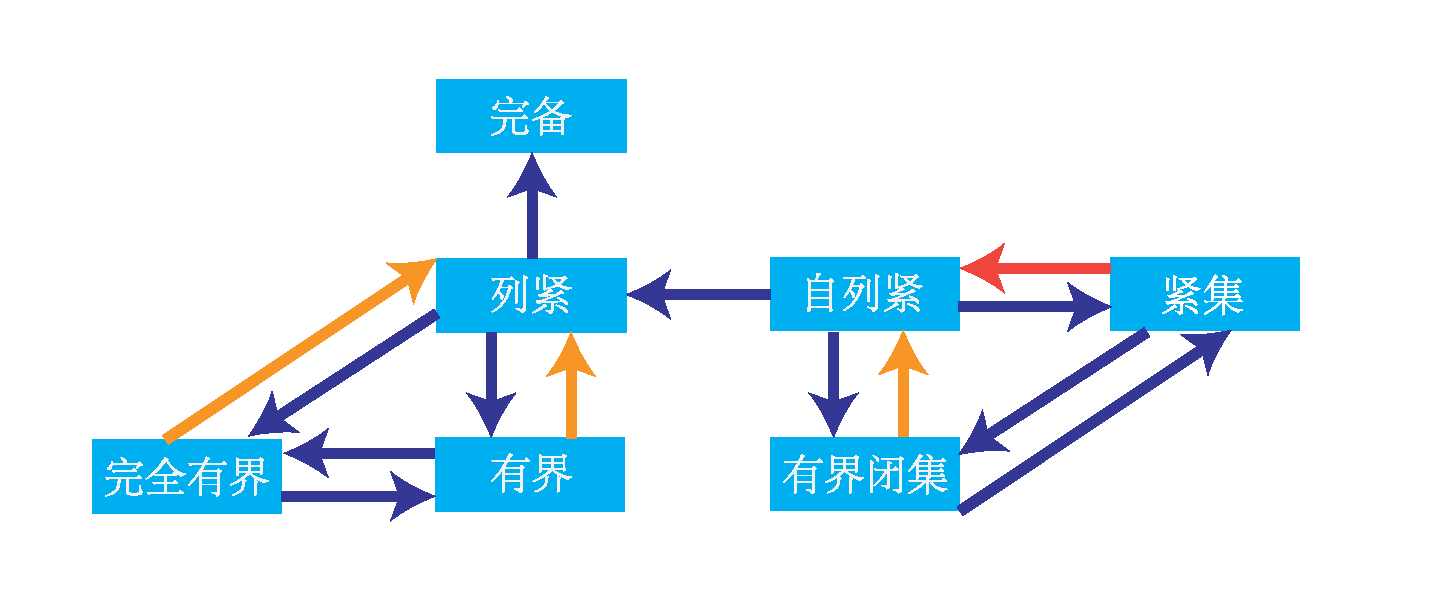
\includegraphics[scale = 0.4]{ideo.pdf}
\end{figure}
类似于实数中的集合,度量空间里也可以引入完备性等概念。

\begin{definition}[基本列]
    度量空间 $(\mathscr{X},d)$ 中的点列叫做基本列指:$d(x_n,x_m)\to0$。也就是说:$\forall\varepsilon,\exists N(\varepsilon)$、当$n,m\ge N(\varepsilon)$ 有 $d(x_n,x_m)\to 0$。如果空间的所有基本列是收敛列,则称该空间是完备的。(\textit{与数学分析中柯西列的定义类似})
\end{definition}
\begin{example}
    $(R^n, d)$是完备的。
\end{example}
\begin{example}
    $(C[a,b],\rho)$是完备的度量空间。
\end{example}
\begin{solution}
    设$x_{n}$是一串基本列,那么$\forall\varepsilon>0,\exists N(\varepsilon)$。使得当 $n,m\geq N(\varepsilon)$ 有 
    \begin{equation*}
        \rho\left(x_{n},x_{m}\right)=\max\limits_{a\leq t\leq b}\left|x_{m}\left(t\right)-x_{n}\left(t\right)\right|\leq\varepsilon
    \end{equation*}
    因此,$\forall t\in[a,b]$,有
    \begin{equation*}
        \left|x_{m}\left(t\right)-x_{n}\left(t\right)\right|\leq\varepsilon.
    \end{equation*}
    现在固定某个$t\in[a,b]$,我们看到$x_n$ 是基本列,由 ($([a,b],|.|)$ 完备性从而极限 $\lim\limits_{n\to\infty}x_n$ 点点存在,记为 $x_0(t)$。在上式中令 $m\to\infty$ 则$\forall n\geq N\left(\varepsilon\right),\left|x_{0}\left(t\right)-x_{n}\left(t\right)\right|\leq\varepsilon$,可见 $x_n(t)$ \textbf{一致收敛}到 $x_0(t)$ ,故 $x_0(t)$ 连续且在$\left(C[a,b],\rho\right)$ 中 $x_n$ 收敛到 $x_0$,即 $\left(C[a,b],\rho\right)$ 是完备的,证毕。
\end{solution}
\bigskip
\begin{definition}[有界]
    给定$\mathscr{X}$是距离空间,$A$是其子集,称$A$是有界的:$\exists x_0\in\mathscr{X},\exists r>0$ 、使得 $A\subset B\left(x_{0},r\right)$。其中,$B\left(x_{0},r\right)=\left\{x\in\mathscr{X}|\rho\left(x,x_{0}\right)<r\right\}.$
\end{definition} 

\textcolor{red}{在有穷维欧式空间里,有界无穷集必有收敛子列,但这不能推广到无穷维空间里。}
\begin{example}
     在$C[0,1]$中,考察点列:记
    \begin{equation}
        \left.x_{n}\left(t\right):=\left(\begin{array}{ll}0&t\geq\frac{1}{n},\\1-nt&0\leq t\leq\frac{1}{n}\end{array}\right.\right). \nonumber
    \end{equation}
    显然$x_n\in B(\zeta, 2)$,$\zeta$(表示恒为0的函数,但在$C[0,1]$中$x_n$没有收敛列,事实上$x_{n}\left(t\right)$逐点收敛于$x\left(t\right)$。
    \begin{equation*}
        x(t) := \left(\begin{array}{ll}
            0 & 0<t\le 1 \\
            1 & t = 0
        \end{array}\right) 
    \end{equation*}
    显然 $x\left(t\right)$ 不是连续函数。
\end{example}

\newpage
\section{列紧集}
\begin{figure}[H]
    \centering
    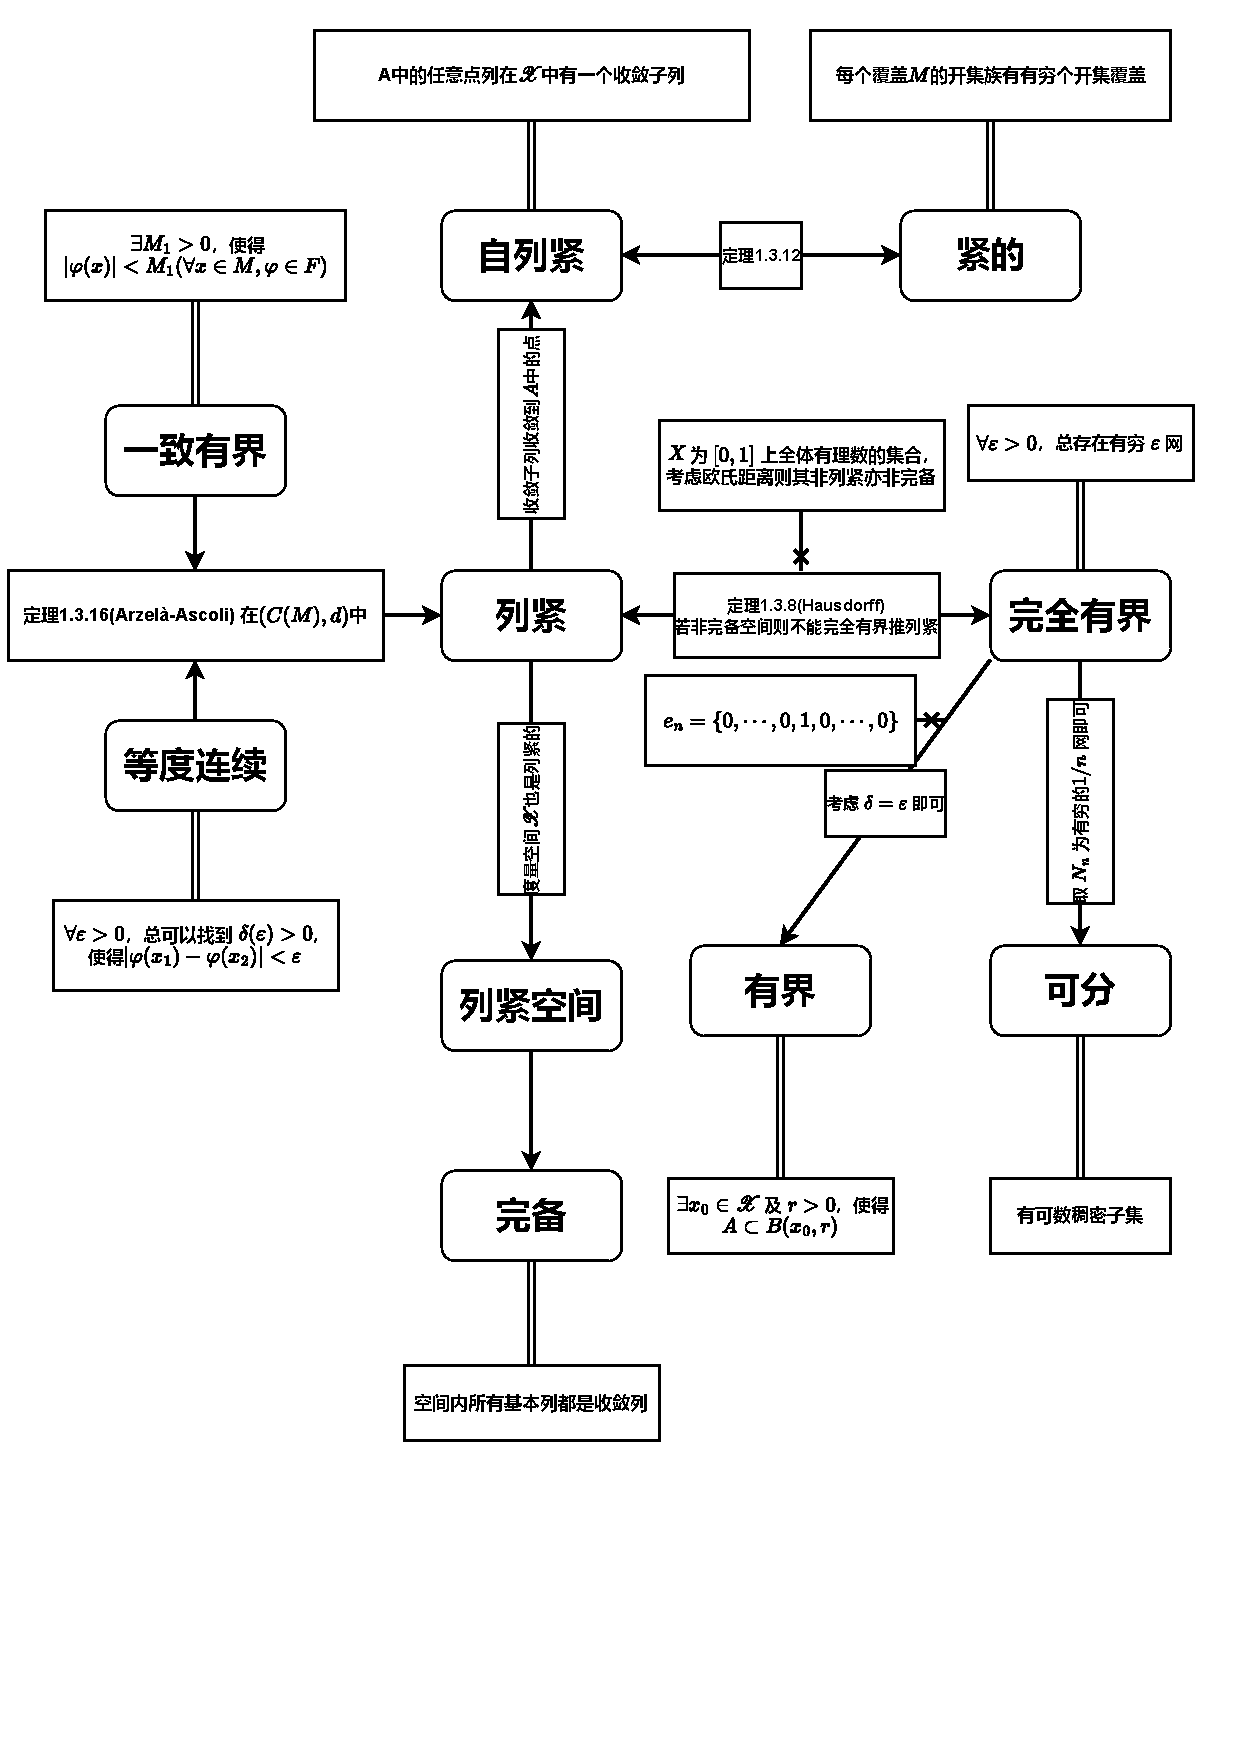
\includegraphics[scale = 0.85, trim = {0cm, 5cm, 0.5cm, 0cm}, clip]{document/functional analysis_1.drawio.pdf}
    \caption{导图}
    \label{fig-1}
\end{figure}

\begin{definition}[自列紧与列紧]
    $(\mathscr{X},\rho)$是距离空间,$A$是其子集,$A$称为列紧的,如果$A$的任何点列都在$\mathscr{X}$中存在收敛子列,若该子列还收敛到$A$中,则A称为自列紧的。若空间$\mathscr{X}$是列紧的,则称$\mathscr{X}$为列紧空间。
\end{definition}
\begin{proposition}
    $R^n$ 中任意有界点列都是列紧的,任意有界闭集都是自列紧的。
\end{proposition}
\begin{proposition}
    列紧空间中任管(闭)子集是(自)列紧的。
\end{proposition}
\begin{proposition}
    列紧集一定是有界的。
\end{proposition}
\begin{solution}
    反证法。假设$A$无界,考虑点列 $\{x_n\}$,s.t. $d(x_n,a)>n$,其中$a\in A$。显然该点列任意子列都是无界的,故无收敛子列,矛盾。
\end{solution}
\begin{proposition}
    列紧空间必是完备空间。
\end{proposition}
\begin{solution}
    $\{\mathscr{X},\rho\}$是列紧空间,设$x_{n}$是其一无穷点列,由列紧性知存在子列
 $x_{n_k}$收敛到点$x_0$,再根据习题1-2-2知$x_n\to x_0$,那么$\{\mathscr{X},\rho\}$是完备空间。
\end{solution}

\begin{theorem}[\textbf{Hausdorff}]
    $\{\mathscr{X},\rho\}$是(完备)度量空间,其子集$M$是列紧的必须(且仅需)$M$是完全有界的。
\end{theorem}
\begin{solution}
    $\Longleftarrow$利用反证法,若$M$没有有穷的 $\varepsilon$ 网,则$\forall\varepsilon_{0}>0,\forall x_{1}\in M,\exists x_{2}\in M\backslash B\left(x_{1},\varepsilon\right)$, 接下来:
\begin{align*}
    & x_{1},x_{2}\in M,\exists x_{3}\in M\setminus\bigcup\limits_{i=1,2}B\left(x_{i},\varepsilon_{0}\right) \\
    & \cdots\cdots\cdots\cdots\cdots\\
    & x_{1},x_{2},...,x_{n}\in M,\exists x_{n+1}\in M\setminus\bigcup\limits_{i=1,\cdots,n+1}B\left(x_{i},\varepsilon_{0}\right).
\end{align*}

如此构造出一点列$x_n$,然而$x_n$不是基本列即$\rho(x_n,x_m)>\varepsilon_0$,这与$M$是列紧的矛盾。

$\Longrightarrow$ 若 $x_n$ 是M 中无穷点列,则对于 1 网,$\exists y_1,x_n^{(1)}$ 是 $x_n$ 的子 列,有$x_{n}^{\left(1\right)}\subset B\left(y_{1},1\right)$, 对于$\frac{1}{2}$网,$\exists y_{2},x_{n}^{(2)}$是$x_{n}^{(1)}$的子列,有$x_{n}^{(2)}\subset B(y_{2},\frac{1}{2})$,
 对于$\frac{1}{n}$网,$\exists y_{n},x_{n}^{(n)}$是$x_{n}^{(n-1)}$的子列,有$x_{n}^{(n)}\subset B(y_{n},\frac{1}{n})$,
 对$x_n^{(n+p)}$取对角线元素,则有$x_n$ 是基本列,事实上

\begin{equation}
\rho\left(x_{n}^{\left(n\right)},x_{n+p}^{\left(n+p\right)}\right)=\rho\left(x_{n}^{\left(n\right)},y_{n}\right)+\rho\left(y_{n},x_{n+p}^{\left(n+p\right)}\right)<\varepsilon.
\end{equation}
再有$(\mathscr{X},\rho)$是完备度量空间得到$M$是列紧的,证毕。
\end{solution}

\bigskip
\begin{definition}[紧集]
    $\{\mathscr{X}, \rho\}$是度量空间,$M$为其子集,$M$称为紧的,当$\mathscr{X}$中任意覆盖$M$的开集族中都有有限个开集覆盖$M$。
\end{definition}
\begin{theorem}
    $\{\mathscr{X},\rho\}$是度量空间,$M$为其子集,$M$是紧的当且仅当$M$是自列紧的。
\end{theorem}
\begin{solution}
    (必要性)设$M$是紧的、先证$M$是闭集,即证$\mathscr{X}/M$是开集, 即证 $\forall x_{0}\in \mathscr{X}/M,\exists r$ 有 $B\left(x_{0},r\right)\cap M=\phi$
    \begin{equation*}
        M\subset\bigcup\limits_{x\in M}B(x,\frac{1}{2}\rho(x,x_{0}))
    \end{equation*}
    由$M$是紧的,则存在$n$和点列$x_{n}$有
    \begin{equation*}
        M\subset\bigcup\limits_{k=1}^{n}B\left(x_{k},\frac{1}{2}\rho\left(x_{k},x_{0}\right)\right).
    \end{equation*} 
    设$\delta:=\frac{1}{2}\min_{1\leq k\leq n}\rho\left(x_{k},x_{0}\right),\forall x\in B\left(x_{0},\delta\right)$,有$\rho\left(x,x_{k}\right)\geq\rho\left(x_{k},x_{0}\right)-\rho\left(x_{0},x\right)\geq\frac{1}{2}\rho\left(x_{k},x_{0}\right)$,所以 $x\notin\bigcup\limits_{k=1}^nB(x_k,\frac{1}{2}\rho(x_k,x_0))$ 即 $B(x_0,\delta)\bigcap M=\phi$,故 $\mathscr{X}/M$ 是开集。

    再证M 是列紧的:反证法:设$M$中的点列 $\{x_n\}$ 不存在收敛子列,不妨假定令 $\{x_n\}$ 互异,再令$S_n:=\{x_1,...,x_{n-1},x_{n+1},...\}$,则$S_n$ 是闭集 (因为不含收敛子列),$\mathscr{X}/\{x_n\}$是开集,则$\bigcup\limits_{n=1}^{\infty}\left(\mathscr{X}/S_{n}\right) = \mathscr{X}/\bigcap\limits_{n=1}^{\infty}S_{n}=\mathscr{X}/\phi=\mathscr{X}\supset M.$

    由M是紧的知存在$N$,使得:$\cup_{n=1}^{N}\left(X/S_{n}\right)=\mathscr{X}/\left\{x_{n}\right\}_{n=N+1}^{\infty}\supset M.$。然而,$\{x_n\}\in M$ 但 $\{x_n\}\notin\mathscr{X}/\{x_n\}_{n=N+1}^{\infty}$,此则导出矛盾,故$M$是列紧的。

    (充分性) 设 $M$ 是自列紧的,要证在覆盖 $M$ 的所有开覆盖中取出有限个覆盖 M。
    反证法: 若某个覆盖族 $U_{\lambda \in A} G_\lambda \supset M$ 中不能取到有限个开覆盖。由 $\mathrm{M}$ 是自列紧的,故完全有界, $\forall n \in N$ 存在有穷 $\frac{1}{n}$ 网:
    $$
    N_n=\left\{x_1^{(n)}, x_2^{(n)}, \ldots, x_{n_k}^{(n)}\right\}, \cup_{y \in N_n} B\left(y_n, \frac{1}{n}\right) \supset M^2 \text { 。 }
    $$

    取 $\left\{y_n\right\} \in N_n$ ,有开球列 $B\left(y_n, \frac{1}{n}\right)$ 不能由有限个 $G_\lambda$ 覆盖。由 $\left\{y_n\right\} \subset M$ 自列紧,故存在收敛子列 $y_{n_k} \rightarrow y_0, y_0 \in G_{\lambda_0}$, 由 $G_{\lambda_0}$ 是开集, $\exists \delta>0$ 有 $B\left(y_0, \delta\right) \in G_{\lambda_0}$, 对此 $\delta$, 令 $k$ 足够大使得 $\frac{1}{n_k}<\frac{\delta}{2}$, 且 $y_{n_k} \in B\left(y_0, \frac{\delta}{2}\right)$, 则对 $\forall x \in B\left(y_{n_k}, \frac{1}{n_k}\right)$ ,有
    $$
    d\left(x, y_{n_k}\right)<d\left(x, y_0\right)+d\left(y_0, y_{n_k}\right) \leq \frac{1}{n_k}+\frac{\delta}{2}<\delta,
    $$

    即 $B\left(y_{n_k}, \frac{1}{n_k}\right) \subset G_{\lambda_0}$ ,这与 $B\left(y_n, \frac{1}{n}\right)$ 不能由有限个 $G_\lambda$ 覆盖矛盾,证毕。
\end{solution}
\begin{center}
    Wed, Mar 6
\end{center}
\begin{center}
    泛函分析中的反例
\end{center}
\begin{remark}
    在不完备的空间之中,列紧可以推出完全有界,但是完全有界无法推出列紧。
\end{remark}

我们曾考虑区间 $[a, b]$ 上的连续函数全体 $C[a, b]$ ,现在稍推广,令 $\mathrm{M}$是紧的距离空间,距离定为 $\rho$ ,用 $C(M)$ 表示 $M$ 上的连续胦射全体: $M \rightarrow R^1$ ,定义距离:
$$
d(u, v):=\max\limits_{t \in M}|u(t)-v(t)|
$$

\begin{proposition}
    $C(M, d)$ 是一个完备的距离空间。
\end{proposition}
\begin{solution}
    只需证明 $C(M)$ 上距离: $d(u, v)$ 的合理性即可,事实上, $u(M)$ 是紧集,因为 $\forall y_n$ in $C(M)$ 都 $\exists x_n \in M$ 有 $u\left(x_n\right)=y_n$ 。由 $M$ 是紧集,即自列紧,
    $y_{n_k}=u\left(x_{n_k}\right) \rightarrow u\left(x_0\right)$, 记 $y_0:=u\left(x_0\right)$ ,故 $u(M)$ 是紧集,在 $R^1$ 上也是有界闭集,设:
    $$
        \min u(M)=a, \quad y\max u(M)=b,
    $$

    则由闭性知 $a, b \in u(M)$ ,这就推出 $\max\limits_{t \in M}|u(t)|$ 是存在的。基于 $M$ 的紧性,完备性很容易证明。
\end{solution}

\begin{definition}[一致有界与等度连续]
    $F$ 是 $C(M)$ 的子集,称 $F$ 是一致有界的,若 $\forall x \in M, \forall \varphi \in F, \exists M_1$ 有 $|\varphi(x)| \leq M_1$.
称 $F$ 是等度连续,若 $\forall \varepsilon>0, \forall x_1, x_2 \in M, \forall \varphi \in F, \exists \delta(\varepsilon)$ ,使得当 $d\left(x_1, x_2\right) \leq \delta(\varepsilon)$ 有 $\left|\varphi\left(x_1\right)-\varphi\left(x_2\right)\right| \leq \varepsilon$.
\end{definition}

接下来我们讨论连续函数空间上紧集的刻画。
\begin{theorem}[Arzelà-Ascoli]
    为了 $F$ 是 $(C(M), d)$ 的列紧集, 必须且仅须 $F$ 是一致有界且等度连续的函数族。
\end{theorem}
\begin{solution}
    因为 $(C(M), d)$ 是完备的, 由定理 3.7 知道, $F$ 是列紧的必须且仅需 $F$是完全有界的。
    
    (必要性) 若 $F$ 是完全有界的,由 $C(M)$ 上距离的定义知 $F$ 是一致有界的。这是因为 $F$ 完全有界,故存在有穷 $\varepsilon / 3$ 网$N_{\varepsilon / 3}=\left\{\phi_1, \phi_2, \cdots, \phi_n\right\}$, 使得 $\forall \phi \in F, \exists \phi_i \in N_{\varepsilon / 3}$, 满足
    $$
        d\left(\phi, \phi_i\right)<\varepsilon / 3 
    $$
    $\forall \phi_i \in C(M), \phi_i(M)$ 有界, 即 $\exists k_i \in \mathbb{R}$, s.t. $\left|\phi_i(x)\right|<k_i, \forall x \in M$.

    令 $k=\max\limits_{1 \leq i \leq n}\left\{k_i\right\}+\varepsilon / 3$.
    $$
        |\phi(x)| \leq\left|\phi(x)-\phi_i(x)\right|+\left|\phi_i(x)\right| \leq k,
    $$
    $\forall x \in M, \forall \phi \in F$. 这说明 $F$ 一致有界.

    下证等度连续:

    由 $F$ 是完全有界知 $F$ 存在有穷的 $\frac{\epsilon}{3}$ 网,记为 $N\left(\frac{\varepsilon}{3}\right)=\left\{\varphi_1, \ldots, \varphi_n\right\}$. 即 $\forall \varphi \in F$ ,存在某个 $\varphi_{i_0}$ 使得:
    $$
        \left|\varphi(x)-\varphi_{i_0}(x)\right| \leq \frac{\varepsilon}{3}, \quad(\forall x \in M) .
    $$

    另一方面对每个网点 $\varphi_i$ 由连续性知对于 $\frac{\varepsilon}{3}$ ,存在公共的 $\delta(\varepsilon)$ 使得当 $d\left(x_1-x_2\right) \leq \delta, \quad\left(\forall x_1, x_2 \in M\right)$ 有
    $$
        \left|\varphi_i\left(x_1\right)-\varphi_i\left(x_2\right)\right| \leq \frac{\varepsilon}{3} .
    $$

    那么对上述的 $\delta(\varepsilon), \forall x_1, x_2 \in M$ ,且 $d\left(x_1, x_2\right) \leq \delta$ 有
    \begin{align*}
        \left|\varphi\left(x_1\right)-\varphi\left(x_2\right)\right| & \leq\left|\varphi\left(x_1\right)-\varphi_{i_0}\left(x_1\right)\right|+\left|\varphi_{i_0}\left(x_1\right)-\varphi_{i_0}\left(x_2\right)\right|+\left|\varphi\left(x_2\right)-\varphi_{i_0}\left(x_2\right)\right| \\
        & \leq \frac{\varepsilon}{3}+\frac{\varepsilon}{3}+\frac{\varepsilon}{3}=\varepsilon
    \end{align*}

    (充分性) $F$ 一致有界且等度连续,要证 $F$ 存在有穷的 $\varepsilon$ 网。首先由 $F$等度连续知 $\forall \varepsilon>0, \forall x_1, x_2 \in M, \forall \varphi \in F, \exists \delta(\varepsilon)$ 有
    $$
        \left|\varphi\left(x_1\right)-\varphi\left(x_2\right)\right| \leq \frac{\varepsilon}{3}, \quad\left(d\left(x_1, x_2\right) \leq \delta\right) .
    $$

    然后对此 $\delta$, 由 $M$ 是紧的知存在有穷的 $\delta$ 网,记为 $N(\delta)=\left\{x_1, x_2, \ldots, x_n\right\}$ ,作映射 $T: F \rightarrow R^n:$
    $$
        T \varphi=\left(\varphi\left(x_1\right), \varphi\left(x_2\right), \ldots \varphi\left(x_n\right)\right) .
    $$

    令 $\bar{F}=T F$ ,因为 $F$ 一致有界 $\left(\max _{x \in M}|\varphi(x)| \leq M_1\right)$ ,则有
    $$
        \left(\sum_{i=1}^n \varphi^2\left(x_i\right)\right)^{\frac{1}{2}} \leq \sqrt{n} M_1
    $$

    故 $\bar{F}$ 在 $R^n$ 中有界,即列紧。再者由定理 1.3.7 知 $\bar{F}$ 完全有界,故存在有穷的 $\frac{\varepsilon}{3}$ 网,记作
    $$
        \bar{N}\left(\frac{\varepsilon}{3}\right)=\left(T \varphi_1, T \varphi_2, \ldots, T \varphi_n\right) .
    $$

    即 $\forall \varphi \in F$ ,存在某个 $\varphi_i$ 使得:
    $$
        d\left(T \varphi, T \varphi_i\right)=\left[\sum_{k=1}^n\left(\varphi\left(x_k\right)-\varphi_i\left(x_k\right)\right)^2\right]^{\frac{1}{2}} \leq \frac{\varepsilon}{3} .
    $$

    最后只需验证 $\left(\varphi_1, \varphi_2, \ldots, \varphi_n\right)$ 是 $F$ 的有穷的 $\varepsilon$ 网即可。$\forall x \in M, \forall \varphi \in F$ ,存在 $\mathrm{M}$ 的某个网点 $x_\tau \in N(\delta)$ 与 $\mathrm{F}$ 的某个网点 $\varphi_i$,使得:
    $$
    \begin{aligned}
        \left|\varphi(x)-\varphi_i(x)\right| & \leq\left|\varphi(x)-\varphi\left(x_r\right)\right|+\left|\varphi\left(x_r\right)-\varphi_i\left(x_r\right)\right|+\left|\varphi_i\left(x_\tau\right)-\varphi_i(x)\right| \\
        & \leq \frac{\varepsilon}{3}+d\left(T \varphi, T \varphi_i\right)+\frac{\varepsilon}{3}=\varepsilon .
    \end{aligned}
    $$
\end{solution}

\begin{example}
    若 $\Omega \in R^n$ 是有界开凸集, $M_1, M_2$ 是给定正数、则集合
    $$
        F:=\left\{\varphi(x) \in C^1(\bar{\Omega})|| \varphi(x)\left|\leq M_1,\right| \operatorname{grad} \varphi(x) \mid \leq M_2\right\}
    $$
    是 $C^1(\bar{\Omega})$ 中的列紧集,其中 $C^1(\bar{\Omega})$ 表示 $\bar{\Omega}$ 连续可微函数全体。
\end{example}
\begin{solution}
    证明: 图为 $\forall x_1, x_2 \in \bar{\Omega}, \varphi \in F, \exists 0<\theta<1$ 使得
    $$
        \left|\varphi\left(x_1\right)-\varphi\left(x_2\right)\right|=\left|\operatorname{grad} \varphi\left(x_1+\theta\left(x_2-x_1\right)\right) d\left(x_2, x_1\right)\right| \leq M_2 d\left(x_2, x_1\right),
    $$
    故 $F$ 等度连续, 易知 $F$ 一致有界, 由定理 1.3.15 知 $F$ 列紧, 证毕。
\end{solution}

定义 1.6
包含是 $(\mathbf{X}, d)$ 的最小完备的度量空间称为 $\mathbf{X}$ 的完备化空间,其中最小的意思是任何包含 $\mathbf{X}, d)$ 的完备度量空间都以 $\mathbf{X}$ 的完备化空间为子集。

命题 1.7
$\left(\mathbf{X}_1, d_1\right)$ 是以 $(\mathbf{X}, d)$ 为子空间的完备度量空间,且 $\left.d_1\right|_{\mathbf{X}_1, \mathbf{X}_1}=d,(\mathbf{X}, d)$在 $\left(\mathbf{X}_1, d_1\right)$ 中稠密, 则 $(\mathbf{X}, d)$ 的完备化空间是 $\left(\mathbf{X}_1, d_1\right)$ 。
证明: $\forall \xi_1 \in \mathbf{X}_1, \exists x_n \in \mathbf{X}$ 有 $d_1\left(x_n, \xi_1\right) \rightarrow 0$ 。若存在完备空间 $\mathbf{X}_2$ 包含 $X$ ,有
$$
d_2\left(x_n, x_m\right)=d_1\left(x_n, x_m\right) \rightarrow 0 .
$$

则存在 $\xi_2 \in \mathbf{X}_2$ ,有 $d_2\left(x_n, \xi_2\right) \rightarrow 0$. 于是作映射 $T: \mathbf{X}_1 \rightarrow \mathbf{X}_2$,
$T \xi_1=\xi_2$. 再证映射 $T$ 是等距的, $\forall \eta_1 \in \mathbf{X}_1, \exists y_n \in \mathbf{X}$ 有 $\rho_1\left(y_n, \eta_1\right) \rightarrow 0$, 则
$$
d_1\left(\xi_1, \eta_1\right)=\lim _{n \rightarrow \infty} d_1\left(x_n, y_n\right)=\lim _{n \rightarrow \infty} d_2\left(x_n, y_n\right)=d_2\left(\xi_2, \eta_2\right) .
$$

如此证明映射 $T$ 是等距的, $\mathbf{X}_1$ 与 $R(T) \subset \mathbf{X}_2$ 等距同构,故 $\mathbf{X}$ 的完备化空间为 $\left(\mathbf{X}_1, d_1\right)$ 。

\newpage
\begin{center}
    Mon, Mar 11
\end{center}
\section{完备化}
\begin{definition}[完备化空间]
    包含在$(X, d)$的最小完备的度量空间称为$X$的完备化空间,其中最小的意思是任何包含$(X, d)$的完备度量空间都以$X$的完备化空间为子集。
\end{definition}

\begin{proposition}
    $\left(\mathbf{X}_1, d_1\right)$ 是以 $(\mathbf{X}, d)$ 为子空间的完备度量空间,且 $\left.d_1\right|_{\mathbf{X}, \mathbf{X}}=d(\mathbf{X}, \mathbf{X}),(\mathbf{X}, d)$在 $\left(\mathbf{X}_1, d_1\right)$ 中稠密, 则 $(\mathbf{X}, d)$ 的完备化空间是 $\left(\mathbf{X}_1, d_1\right)$ 。
    \begin{center}
        \begin{tabular}{ccccc}
        $\overline{(\mathbf{X}, d)}$ & $\subset$ & $(\mathbf{X}_1, d_1)$ & $\subset$ & $(\mathbf{Y}, \Tilde{d})$  \\
        & & 完备化 & & 完备 \\
        \end{tabular}
    \end{center}
    \begin{align*}
        d_1: \mathbf{X}\cdot \mathbf{X} = d(\mathbf{X}, \mathbf{X}) \\
        \left\lbrace\begin{array}{cc}
        (\overline{\mathbf{X}}, d) &\supset (\mathbf{X}_1, d_1)  \\
        (\mathbf{X}, d) &\subset (\mathbf{X}_1, d_1) 
        \end{array} \right.
    \end{align*}
\end{proposition}
\begin{solution}
    $\forall \xi_1 \in \mathbf{X}_1, \exists x_n \in \mathbf{X}$ 有 $d_1\left(x_n, \xi_1\right) \rightarrow 0$ 。若存在完备空间 $\mathbf{X}_2$ 包含 $\mathbf{X}$, 有
    \begin{align*}
        d_2\left(x_n, x_m\right)=d\left(x_n, x_m\right) \rightarrow 0
    \end{align*}

    则存在 $\xi_2 \in \mathbf{X}_2$, 有 $d_2\left(x_n, \xi_2\right) \rightarrow 0$. 于是作映射 $T: \mathbf{X}_1 \rightarrow \mathbf{X}_2$, $T \xi_1=\xi_2$. 再证映射 $T$ 是等距的, $\forall \eta_1 \in \mathbf{X}_1, \exists y_n \in \mathbf{X}$ 有 $\rho_1\left(y_n, \eta_1\right) \rightarrow 0$, 则
    \begin{align*}
        d_1\left(\xi_1, \eta_1\right)=\lim\limits_{n \rightarrow \infty} d_1\left(x_n, y_n\right)=\lim\limits_{n \rightarrow \infty} d_2\left(x_n, y_n\right)=d_2\left(\xi_2, \eta_2\right) = d_2(T\xi_1, T\eta_1)
    \end{align*}

    如此证明映射 $T$ 是等距的, $\mathbf{X}_1$ 与 $R(T) \subset \mathbf{X}_2$ 等距同构,故 $\mathbf{X}$ 的完备化空间为 $\left(\mathbf{X}_1, d_1\right)$ 。
\end{solution}

\begin{theorem}
    每个度量空间都有完备化空间。
\end{theorem}
\begin{solution}
    设 $(\mathbf{X}, d)$ 是度量空间,以下分三步证明:
    
    (1) 把 $(\mathbf{X}, d)$ 中的基本列 $\left\{x_n\right\}$ 分类,凡是满足:
    \begin{align*}
        \lim\limits_{n \rightarrow 0} d\left(x_n, y_n\right)=0
    \end{align*}
    称他们是等价的,把等价的点列 $\left\{x_n\right\},\left\{y_n\right\}$ 都归做一类(等价类)。设 $\left(\mathbf{X}_1, d_1\right)$ 是以 $(\mathbf{X}, d)$ 中的等价类构成的度量空间,定义距离:$\forall \xi, \eta \in \mathbf{X}_1$,任取 $\left\{x_n\right\} \in \xi,\left\{y_n\right\} \in \eta$,
    \begin{align*}
        d_1(\xi, \eta)=\lim\limits_{n \rightarrow 0} d\left(x_n, y_n\right) .
    \end{align*}
    
    由实数的完备性知道上面的极限是可以取到的。以下证明上式是距离,按照距离定义,(1) 和 (2) 都是显然的,而 (3)可由
    \begin{align*}
        d\left(x_n, y_n\right) \leq d\left(x_n, z_n\right)+d\left(z_n, y_n\right)
    \end{align*}

    取极限得到, 则能证明 $(\left.\mathbf{X}_1, d_1\right)$ 是个距离空间。
    
    (2) $\forall x \in \mathbf{X}$,定义 $\xi_x=\{x, x, \ldots, x\}$ ,并以此 $\xi_x$ 构成距离空间 $\left(\mathbf{X}^{\prime}, d_1\right)$ ,显然有 $\mathbf{X}^{\prime} \subset \mathbf{X}_1$。定义 $T: \mathbf{X} \rightarrow \mathbf{X}^{\prime}$ 的映射, $T x=\xi_x$, 容易验证 $T$ 是等距映射,故 $(\mathbf{X}, d)$ 与 $\left(\mathbf{X}^{\prime}, d_1\right)$ 等距同构。
    
    接着再证明 $\mathbf{X}^{\prime}$ 在 $\mathbf{X}_1$ 中是稠密的: $\forall \xi=\left\{x_k\right\} \in \mathbf{X}_1$,其中 $\left\{x_k\right\}$ 取为基本列(这里使用基本列则意味着下方的$n$可被$\varepsilon$控制)。$\exists x_n \in \mathbf{X}$,和 $\xi_x=\left\{x_n, \ldots, x_n\right\} \in \mathbf{X}^{\prime}$(选择所有元素均一致的点列),满足
    \begin{align*}
        d_1\left(\xi, \xi_x\right)=\lim\limits_{k \rightarrow \infty} d\left(x_k, x_n\right)<\varepsilon
    \end{align*}

    则有$\mathbf{X}^{\prime}$ 在 $\mathbf{X}_1$ 中是稠密的。

    (3) 最后证明 $\left(\mathbf{X}_1, d_1\right)$ 是完备的,即 $\forall\left\{\xi_n\right\} \in \mathbf{X}_1$ 是基本列,存在 $\xi \in \mathbf{X}_1$ 有:
    \begin{align*}
        \lim\limits_{n \rightarrow \infty} d_1\left(\xi, \xi_n\right) \rightarrow 0
    \end{align*}

    因为 $\mathbf{X}^{\prime}$ 在 $\mathbf{X}_{\mathbf{1}}$ 中稠密,所以对于任意的 $\xi_n, \exists \eta_n=\left\{y_n, \cdots, y_n\right\} \in \mathbf{X}^{\prime}$ ,满足 $d_1\left(\xi_n, \eta_n\right)<1 / n, n=1,2,3, \cdots$.

    首先 $\eta_n$ 是 $\left(\mathbf{X}^{\prime}, d_1\right)$ 中基本列,因为
    \begin{align*}
        d_1\left(\eta_n, \eta_m\right) \leq d_1\left(\eta_n, \xi_n\right)+d_1\left(\xi_n, \xi_m\right)+d_1\left(\xi_m, \eta_m\right)<1 / n+d_1\left(\xi_n, \xi_m\right)+1 / m \text {. }
    \end{align*}

    这同时说明 $\left\{y_n\right\}$ 是 $(\mathbf{X}, d)$ 中基本列。
    
    其次令 $\xi=\left\{y_1, y_2, \cdots\right\}$, 则根据定义 $\xi \in \mathbf{X}_1$, 且有 $\lim\limits_{n \rightarrow \infty} \eta_n=\xi$, 这是因为
    \begin{align*}
        d_1\left(\xi, \eta_n\right)=\lim\limits_{k \rightarrow \infty} d\left(y_k, y_n\right) \rightarrow 0
    \end{align*}

    最后只需证明 $\lim\limits_{n \rightarrow \infty} \xi_n=\xi$ 即可。因为
    \begin{align*}
        d_1\left(\xi, \xi_n\right) \leq d_1\left(\xi, \eta_n\right)+d_1\left(\eta_n, \xi_n\right) \leq d_1\left(\xi, \eta_n\right)+1 / n \rightarrow 0
    \end{align*}
\end{solution}

\section{不动点}
设$\phi(x)$是$\mathbb{R}\to \mathbb{R}$的实函数,求根:
\begin{equation}
    \phi(x) = 0
\end{equation}
可以转化为求映射
\begin{equation}
    f(x) = x - \phi(x)
\end{equation}
的不动点问题,即求$x\in R$
\begin{equation}
    f(x) = x
\end{equation}

下列常微分方程:
\begin{align}
    \left\{\begin{array}{l}
    \frac{d}{d t} x=F(t, x) \\
    x(0)=\xi
    \end{array}\right.
\end{align}

即求连续函数 $x(t)$ 满足:
\begin{align}
    x(t)=\xi+\int_0^t F(s, x(s)) d s,
\end{align}

也可以看成一个不动点的问题, 为此考察$t$的关于原点的某个领域$[-h, h]$, 在$\mathbb{C}[-h, h]$ 里考虑不动点问题:
\begin{align}
    (T x)(t)=\xi+\int_0^t F(s, x(s)) d s
\end{align}

\begin{example}
    设 $\mathbf{X}=[0,1], T(x)$ 是 $[0,1]$ 上的可微函数,如果:
    \begin{align*}
        \begin{gathered}
            T(x) \in[0,1] \\
            \left|T^{\prime}(x)\right| \leq a<1 .
        \end{gathered}
    \end{align*}
则$T(x)$是压缩映像。
\end{example}
\begin{solution}
    \begin{align*}
        \begin{aligned}
            d(T x, T y) & =|T x-T y| \\
            & =\left|T^{\prime}(x+\theta(y-x))\right||x-y| \\
            & \leq a|x-y| \quad(x, y) \in[0,1]
        \end{aligned}
    \end{align*}
启发设 $T(x):[0,1] \rightarrow[0,1]$ 可微且符合 (10) 和 (11), 则 $T$ 是否存在不动点? 若存在则存在多少个?
\end{solution}

$\forall x_0\in[0, 1]$,作迭代序列$x_{n+1} = Tx_n$,则
\begin{align}
    |x_{n+1} - x_n| & = |Tx_n, Tx_{n-1}| \nonumber\\
    &\leqslant a|x_n - x_{n-1}|\nonumber \\
    &\leqslant a^n|x_1-x_0|
\end{align}

则有
\begin{align}
    |x_{n+p} - x_n| &= |\sum\limits_{i=1}^p (x_{n+i} - x_{n+i-1})| \nonumber\\
    & \leqslant \sum\limits_{i=1}^p a^{n+i-1}|x_1-x_0| \nonumber \\
    & \leqslant \sum\limits_{i=1}^{\infty} a^{n+i-1} |x_1 - x_0| \nonumber \\
    & \leqslant\lim\limits_{n\to\infty} \frac{a^n}{1-a}|x_1 - x_0| \to 0
\end{align}
上式也说明了$\{x_n\}$为一基本列。而由$([0, 1], |\cdot|)$的完备性知极限存在,记为$x^*$。则
\begin{align*}
    x^* = Tx^*
\end{align*}
再证明此不动点唯一:
\begin{align*}
    |x^* - x^{**}| &= |Tx^* - Tx^{**}|\\
    & \leqslant a|x^* - x^{**}|
\end{align*}
由$a<1$知,$x^{*} = x^{**}$,则唯一性证毕。
\begin{theorem}[Banach不动点原理——压缩映像原理]
    设 $(\mathbf{X}, d)$ 是完备的距离空间,若 $T:(\mathbf{X}, d) \rightarrow(\mathbf{X}, d)$ 是压缩映像,则 $T$存在唯一不动点。
\end{theorem}
\begin{solution}
    若 $T:(\mathbf{X}, d) \rightarrow(\mathbf{X}, d)$ 是压缩映射, $\forall x_0 \in \mathbf{X}$ ,考虑迭代序列:
    \begin{align*}
        x_{n+1}=T x_n
    \end{align*}

    跟前面一样我们有:
    \begin{align*}
        \begin{gathered}
            d\left(x_{n+1}, x_n\right)=d\left(T x_{n+1}, T x_n\right) \leq a d\left(x_n, x_{n-1}\right) \leq \ldots \leq a^n d\left(x_1, x_0\right), \\
            d\left(x_{n+p}, x_n\right)=\sum_{i=1}^p d\left(T x_{n+i}, T x_{n+i-1}\right) \leq \frac{a^n}{1-a} d\left(x_1, x_0\right) \rightarrow 0 .
        \end{gathered}
    \end{align*}

    由此可见, $x_n$ 是一个基本列。因为 $(\mathbf{X}, d)$ 是完备的,极限存在且唯一。
    
    在压缩映像原理中,空间的完备性是不可以省略的。例如 $T x:=\frac{1}{2}(1+x)$在 $[0,1]$ 上有唯一不动点 $x_0=\frac{17+1}{8}$ ,然而若取 $\mathbf{X}=[0,1] \backslash x_0$ ,那么 $T$仍然是 $\mathbf{X} \rightarrow \mathbf{X}$ 上的压缩映像,但它没有不动点。
\end{solution}

下列常微分方程
\begin{equation}
    \left\lbrace\begin{array}{ll}
    \frac{d}{dt}x &= F(t, x)  \\
    x(0) &= \xi 
    \end{array}\right.\label{ode-1}
\end{equation}
即求连续函数$x(t)$满足
\begin{align*}
    x(t) = \xi + \int_{0}^t F(s, x(s)) ds
\end{align*}
也可以看成一个不动点问题
\begin{align*}
    (Tx)(t) = \xi + \int_0^t F(s, x(s))ds
\end{align*}
\begin{example}
    常微分方程(\ref{ode-1})的初值问题存在唯一的局部解。
    
    我们把此问题化成不动点问题,先在 $C[-h, h]$ 上考查定义的映射 $T$ ,看看需要添加什么条件使得 $T$ 成为压缩映像:
    \begin{align*}
        \begin{aligned}
            |d(T x, T y)| & =\max _{-h \leq t \leq h}\left|\int_0^t F(s, x(s))-F(s, y(s)) d s\right| \\
            & \leq h \max _{-h \leq t \leq h}|F(s, x(s))-F(s, y(s))| .
        \end{aligned}
    \end{align*}

    因此,比如说令二元函数 $F(t, x)$ 对变元 $\times$ 关于 $\mathrm{t}$ 有一致 Lipschitz 条件: $\exists \delta, L$ 使得对 $\forall|t| \leq h$ 当 $|x-\xi| \leq \delta,|y-\xi| \leq \delta$ 都有:
    \begin{align}
        |F(t, x)-F(t, y)| \leq L|x-y|\label{lipschitz}
    \end{align}

    这时就有:
    \begin{align*}
        d(T x, T y) \leq l h \cdot d(x, y) \quad(x, y) \in \bar{B}(\xi, \delta) .
    \end{align*}

    其中, $\bar{B}(\xi, \delta):=\left\{x(t) \in C[-h, h]\left|\max _{-h \leq i \leq h}\right| x(t)-\xi \mid \leq \delta\right\}$.

    然而,当 $L h<1$ 时, $T$ 只是在 $C[-h, h]$ 的子集 $\bar{B}(\xi, \delta)$ 上是压缩的,这里我们把常数 $\xi$ 看成是 $C[-h, h]$ 中的常值函数。

    我们取 $\mathbf{X}=\bar{B}(\xi, \delta)$ ,要使 $T: \mathbf{X} \rightarrow \mathbf{X}$, 令
    \begin{align*}
        M:=\max \{\mid F(t, x) \|(t, x) \in[-h, h] *[\xi-\delta, \xi+\delta]\} .
    \end{align*}
    则当 $h$ 充分小时有
    \begin{align*}
        \max |T x-\xi|=\max \left|\int_0^t F(s, x) d s\right| \leq h M \leq \delta .
    \end{align*}
    由于 $C[-h, h]$ 完备,而 $\bar{B}(\xi, \delta)$ 是它的闭子集,由于完备的度量空间的闭子集也完备,故我们可以对 $\bar{B}(\xi, \delta)$ 使用压缩不动点定理。
\end{example}

\begin{theorem}
    设函数 $F(t, x)$ 在 $[-h, h] *[\xi-\delta, \xi+\delta]$ 符合 (\ref{lipschitz}),则当 $h<\min \left\{\frac{\delta}{M}, \frac{1}{L}\right\}$ 时, 初值问题 (\ref{ode-1}) 在 $[-h, h]$ 存在唯一解。
\end{theorem}

\section{赋范线性空间}
\subsection{向量空间}
我们在分析中遇到的空间,不仅需要考察收敛性,元素间的代数运算也需要考察,故我们既要研究空间的拓扑结构,也要研究代数结构。
\begin{definition}
    设 $\mathrm{X}$ 是一个非空集, $\mathbb{K}$ 是复 (或实) 数域,如果下列条件满足,便称 $\mathbf{X}$ 是复 (或实) 线性空间。(1) $\mathbf{X}$ 是一加法交换群,即
    
    $\forall x, y \in \mathbf{X}, \exists u \in \mathbf{X}$ ,记 $u=x+y$ 称为 $x, y$ 的和,适合:
    
    (1.1) $x+y=y+x$,
    
    (1.2) $(x+y)+z=y+(x+z)$,
    
    (1.3) 存在唯一的 $\theta \in \mathbf{X}$, 使得 $x+\theta=x$,

    (1.4) $\forall x \in \mathbf{X}$ ,存在唯一的 $x^{\prime} \in \mathbf{X}$ ,使得 $x+x^{\prime}=\theta$ ,记此 $x^{\prime}$ 为 $-x$.
    
    (2) $\forall(a, x) \in \mathbb{K} * \mathbb{X}, \exists \mid u \in \mathbb{K}$ ,记做 $u=a x$ 称为 $a$ 对 $x$ 的数乘。
    
    (2.1) $a(b x)=b(a x) \quad(\forall a, b \in \mathbb{K})$,
    
    (2.2) $1 * x=x_0$

    (2.3) $(a+b) x=a x+b x \quad(\forall a, b \in \mathbb{K}, x \in \mathbf{X})$,
    
    (1.2) $a(x+y)=a x+a y \quad(\forall a, \in \mathbb{K}, x, y \in \mathbf{X})$.

    线性空间的元素称为向量,所以线性空间也称为向量空间。
\end{definition}

\begin{definition}
    设 $\mathbf{X}, \mathbf{X}_1$ 都是线性空间,映射 $T: \mathbf{X} \rightarrow \mathbf{X}_1$ 称为线性同构,如果;

    (1) $T$ 既是单射也是满射,即 $T$ 是一对一旦在上的;

    (2) $T(a x+b y)=a T(x)+b T(y), \quad \forall x, y \in \mathbf{X}$ 。
\end{definition}

\begin{definition}
    $E \subset \mathbf{X}$, 且 $E$ 依 $\mathbf{X}$ 的加法和乘法构成线性空间,则称 $E$为 $\mathbf{X}$ 的线性子空间。$\mathbf{X}$ 和 $\phi$ 都是 $\mathbf{X}$ 的线性子空间,称他们为平凡子空间,其余的线性子空间称为真子空间。
\end{definition}

\begin{definition}
    设 $E \subset \mathbf{X}$ ,若 $\exists x_0 \in \mathbf{X}$ 以及线性子空间 $E_0 \subset \mathbf{X}$ 使得 $E=E_0+x_0:=\left\{x+x_0 \mid x \in E\right\}$, 则称 $\mathrm{E}$ 是 $\mathbf{X}$ 的线性子流形, 可以说线性子流形是线性子空间对于某一向量的平移。
\end{definition}

\begin{definition}
    一组向量 $x_1, x_2, \ldots, x_n$ 称为线性相关的,如果存在不全为零的系数 $k_1, k_2, \ldots, k_n \in \mathbb{K}$,使得: $k_1 x_1+k_2 x_2+\ldots+k_n x_n=0$, 反之则称为线性无关的。
\end{definition}

\begin{center}
    Lundi, Mars 18
\end{center}

\subsection{准范数和范数}
\begin{definition}
    准范数和范数:
    \par\noindent\textbf{准范数:} 正定性、三角不等式、对称性与数乘连续性。$F^*\Longrightarrow F$

    \par\noindent\textbf{范数:} 正定性、三角不等式、齐次性。$B^*\Longrightarrow B$
\end{definition}

\begin{example}
    空间$S$表示一切序列组成的线性空间,按照
    \begin{align*}
        \|x\| = \sum\limits_{i=1}^{\infty} \frac{1}{2^n} \frac{|x_n|}{1+|x_n|}
    \end{align*}
    定义一个准范数,下面我们来说明其为一$F$空间。
\end{example}
\begin{proof}
    我们首先验证其为一准范数。正定性与对称性显然,而对于三角不等式
    \begin{align*}
        \|x+y\| = \sum\limits_{n=1}^{\infty} \frac{1}{2^n} \frac{|x+y|}{1+|x+y|} \le \sum\limits_{i=1}^{\infty}\frac{1}{2^n} \frac{|x| + |y|}{1+|x|+|y|} \le \sum\limits_{i=1}^{\infty} \frac{1}{2^n}\frac{|x|}{1+|x|} + \frac{1}{2^n}\frac{|y|}{1+|y|}  = \|x\| + \| y\|
    \end{align*}

    再证其满足数乘连续性:$\forall a\in\mathbb{K}$,若$\|x_n\|\to 0$则$\|ax_n\|\to 0$。若$\|a_n\|\to 0$,则$\forall\varepsilon/2>0$,$\exists n_0$足够大使得$\frac{1}{2^{x_0}}\le \varepsilon/2$,固定此$n_0$,取$N = N(\varepsilon/2)$,当$m>N$时有$a_m\max\limits_{1\le i\le n_0} x_i\le \varepsilon/2$,则
    \begin{align*}
        \|a_mx\| = \sum\limits_{n=1}^{\infty} \frac{1}{2^n} \frac{|a_mx_n|}{1+|a_mx_n|}\le \sum\limits_{n=1}^{\infty} \frac{1}{2^n}|a_mx_n| + \sum\limits_{n=n_0+1}^{\infty} \frac{1}{2^n} = \varepsilon/2 + \varepsilon/2 = \varepsilon    
    \end{align*}
    故而为一准范数,下面验证完备性,若
    \begin{align*}
        \|x^{m+p} - x^m\| = \sum\limits_{n=1}^{\infty} \frac{1}{2^n} \frac{|x_n^{m+p} - x_n^m|}{1 + |x_n^{m+p} - x_n^m|} < \infty
    \end{align*}
    故而$\forall n\in\mathbb{K}$, $|x_n^{m+p} - x_n^m| \to 0$。又有$\mathbb{R}^n$完备性知,$\exists x^*_n$,使得$|x^m - x_n^*| \to 0$,那么$\forall \varepsilon/2 > 0$,$\exists n_0$足够大的时候使得$\frac{1}{2^{n_0}}\le \varepsilon/2$,固定此$n_0$,取$N = N(\frac{\varepsilon}{2})$,当$m>N$时有$|x_n^m - x_n^*| \le\frac{\varepsilon}{2}$,则
    \begin{align*}
        \|x^m - x_n^*\| = \sum\limits_{i=1}^n \frac{1}{2^n} \frac{|x^m+x^*_n|}{1+|x^m+x_n^*|} < \varepsilon
    \end{align*}
    即构成了一个完备的空间,即$F$空间。
\end{proof}

\begin{example}
    $L^p(\Omega, \mu)$,($1\le p<\infty$) 为范数且完备。
\end{example}

\begin{proposition}
    $L^p$是完备空间。
\end{proposition}

\begin{proof}
    在数学分析中我们就见到过用Bolzano-Weierstrass定理证明Cauchy收敛原理,要证明 $L^p$ 完备,我们只需要证明从任何一个柯西列中都可以选出一个收敛子列。

    设 $\left\{f_n\right\}$ 是 $L^p$ 中的一个柯西列,则根据定义,可以选出指标 $1 \leq n_1 \leq \ldots \leq n_l \leq \ldots$, 使得$\left\|f_{n_{k+1}}-f_{n_k}\right\|_p \leq \frac{1}{2^{k+1}}, \forall k$。

    我们期望序列 $\left\{f_{n_k}\right\}$ 收敛,而这并不难证明。将序列写成和式:$f_{n_k}=f_{n_1}+\sum\limits_{i=1}^{k-1}\left(f_{n_{i+1}}-f_{n_i}\right)$,考虑证明级数绝对收敛。
    
    考察无穷级数 $g_k=\left|f_{n_1}\right|+\sum_{i=1}^k\left|f_{n_{i+1}}-f_{n_i}\right| \geq f_k$, 用三角不等式:
    \begin{align*}
        \left\|g_k\right\|_p \leq\left\|f_{n_1}\right\|_p+\sum_{k=1}^k\left\|f_{n_{k+1}}-f_{n_k}\right\|_p<1+\left\|f_{n_1}\right\|_{p}
    \end{align*}
一致有界,故 $g_k \in L^p$ 。
    
    由 Levi单调收敛定理: $g_k \rightarrow g \in L^p(X)$ 。令 $f=f_{n_1}+\sum_{i=1}^{\infty}\left(f_{n_{i+1}}-f_{n_i}\right)$ 则 $|f| \leq g$ 。由于 $\left|f_{n_k}-g\right|^p \leq|2 g|^p$ ,由Lebesgue控制收敛定理得到 $\left\|f_{n_k}-f\right\|_p \rightarrow 0$。

    这样就找到了一个收敛子列,再用三角不等式就可以简单地完成证明。综上我们证明了性质: $1 \leq p<\infty \Rightarrow L^p$ 是 Banach 空间。
\end{proof}

\begin{remark}
    $L^p(\Omega, \mu)$按通常的加法与数乘规定运算,并且把几乎处处相等的两个函数看作是同一个向量,经这样处理的空间仍然是一个线性空间,并且定义:
    \begin{align}
        \|u\| = \left( \int_{\Omega} |u(x)|^p d\mu\right)^{\frac{1}{p}} \nonumber
    \end{align}
    那么$\|\cdot\|$是一个范数。其中(1)与(3)都是显然的,而(2)是\textsc{Minkowski}不等式推出的。下面证明该不等式。
\end{remark}

我们通过\textsc{Young}不等式推导\textsc{Hölder}不等式,而后得到\textsc{Minkowski}不等式。

\begin{theorem}
    Young Inequality: $\forall a, b\in\mathbb{R}$,我们有
    \begin{align*}
        |a||b| \le \frac{|a|^p}{p} + \frac{|b|^q}{q}, \quad \frac{1}{p} + \frac{1}{q} = 1, \quad 1<p<\infty
    \end{align*}
\end{theorem}

\begin{proof}
    考虑函数$\log x$在$x>0$是凹函数 (concave),则$\forall 0<x_1<x_2$,$\forall 0<\theta<1$,都有
    \begin{align*}
        \log\left( (1-\theta)x_1 + \theta x_2\right) &\ge (1-\theta) \log x_1 + \theta \log x_2\\
        (1-\theta)x_1 + \theta x_2 &\ge x_1^{1-\theta} x_2^{\theta} 
    \end{align*}

    我们令$x_1^{1-\theta} = |a|$,令$x_2^{\theta} = |b|$。其中令$p=\frac{1}{1-\theta}$,$q = \frac{1}{\theta}$。则有
    \begin{align*}
        |a||b|\le \frac{|a|^p}{p} + \frac{|b|^q}{q}
    \end{align*}
    且显然满足上述要求。
\end{proof}

现在我们来用\textsc{Young Ineq}来证明\textsc{Hölder Ineq}。
\begin{theorem}
    \begin{align*}
        \textsc{Hölder Ineq:}\quad \int_E |f(x)| |g(x)| dx\le \|f(x)\|_p\|g(x)\|_q, \quad \frac{1}{p} + \frac{1}{q} = 1, \quad 1\le p \le \infty
    \end{align*}
\end{theorem}

\begin{proof}
    我们可以先证明$p, q$有一为$\infty$时显然成立,故而我们仅证明$1 < p < \infty$即可。
    \begin{align*}
        \int_{E} \left(\frac{|f(x)|}{\|f(x)\|_p}\cdot \frac{|g(x)|}{\|g(x)\|_q} \right)dx \underset{\text{Young Ineq}}{\le} \int_E \frac{\|f(x)\|_p}{p\|f(x)\|_p} dx + \int_E \frac{\|g(x)\|_q}{q\|g(x)\|_q}dx = \frac{1}{p} + \frac{1}{q} = 1\\
    \end{align*}
    因此我们有
    \begin{align*}
        \int_E |f(x)| |g(x)| dx\le \|f(x)\|_p\|g(x)\|_q, \quad \frac{1}{p} + \frac{1}{q} = 1, \quad 1\le p \le \infty
    \end{align*}
\end{proof}

\begin{theorem}
    \begin{align*}
        \textsc{Minkowski}\quad \|f+g\|_p \le \|f\|_p + \|g\|_p \quad 1\le p \le \infty
    \end{align*}
\end{theorem}

\begin{proof}
    Constrain to: $1<p<\infty$,$\|f\|_p<\infty$,
    \begin{align*}
        \|f+g\|_p^p &= \int_E |f(x) + g(x)|^p dx = \int_E |f(x) + g(x)|^{p-1}(f(x) + g(x))dx \\
        \|f+g\|_p^p &\le \underbrace{\int_E \underbrace{|f(x)+g(x)|^{p-1}}\limits_{\textsc{Part I}} \underbrace{|f(x)|}\limits_{\textsc{Part II}} dx}\limits_{I} + \underbrace{\int_{E} |f(x) + g(x)|^{p-1} |g(x)| dx}\limits_{J}
    \end{align*}
\end{proof}

\begin{theorem}
    \textsc{广义的Minkowski:} $1\le p< \infty$,若$\forall j = 1, 2,\cdots$,$f_j\in L^p(E)$,则
    \begin{align*}
       &\sum\limits_{j} |f_j| \in L^p(E) \\
       \text{且} &\quad \| \sum\limits_{j=1}^{\infty} |f_j| \|_p \le \sum\limits_{j=1}^{\infty} \|f_j\|_p
    \end{align*}
\end{theorem}

\begin{example}
    Sobolev 空间:
    \begin{align*}
        \int_{\Omega} \mu\cdot \phi dx_1 = (1-)^k \int_{\Omega} u\cdots \frac{\partial^k \phi}{\partial x_1^k} dx_1
    \end{align*}
    其中$\phi\in C^k(\bar{\Omega})$,$v:= \frac{\partial^k u}{ x_1^k\partial}$称为弱导数。但是该空间$C^m(\bar{\Omega})$是不完备的。将其完备化
    \begin{align*}
        S\triangleq \{ u\in\underset{\text{弱导数}}{C^m(\Omega)} | \|u\|_{m, p} < \infty\}
    \end{align*}
\end{example}

\section{习题部分}
\subsection{习题1}
\begin{remark}
    在度量空间下的闭集,聚点均在集合之中。

    对于度量空间中的连续刻画,采用$\rho$来决定二者的距离。
\end{remark}
\begin{exercise}
    证明:完备空间的闭子集是一个完备的子空间,而任一度量空间中的完备子空间必是闭子集。
\end{exercise}
\begin{proof}
    考虑完备空间$\mathscr{X}$的一个闭子集$M\subseteq \mathscr{X}$,我们要证明其基本列均是收敛列。对于任意基本列$\{x_n\}$,其属于完备空间$\mathscr{X}$,故而必为收敛列。即为完备的。
    
    而由于在度量空间下闭子集之性质,收敛列均收敛于闭集中,故而$M$亦然为完备的子空间。
\end{proof}

\begin{exercise}
    Newton 法
\end{exercise}
\begin{proof}
    我们作一序列$Tx = x - \frac{f(x)}{f^{\prime}(x)}$。考虑其导数
    \begin{align*}
        \frac{d}{dx} Tx &= 1 - \frac{f^{\prime^2}(x) - f(x)f^{\prime\prime}(x)}{f^{\prime^2}(x)} = \frac{f(x)f^{\prime\prime}(x)}{f^{\prime^2}(x)}
    \end{align*}
    而由于$f(\hat{x}) = 0$,$f^{\prime}(\hat{x}) \neq 0$,则
    \begin{align*}
        \frac{d}{dx}\bigg|_{x\to\hat{x}} Tx = 0
    \end{align*}
    故而必然存在一邻域$U(\hat{x})$,使得$\frac{f(x)f^{\prime\prime}(x)}{f^{\prime^2}(x)}\leq \alpha <1$,故而$Tx$为一个压缩映射。
    
    由压缩映射原理,存在不动点$x^*$,使得
    \begin{align*}
        Tx^* = x^*
    \end{align*}
    而由于$\hat{x}$也满足不动点,故而$x^* = \hat{x}$。故而有
    \begin{align*}
        \lim\limits_{n\to\infty} x_n = \hat{x}
    \end{align*}
\end{proof}

\begin{exercise}
    证明不动点唯一
\end{exercise}
\begin{proof}
    由于$\rho(Tx, Ty) < \rho(x, y)$,故而必然存在一个$\delta > 0$,$\rho(Tx, Ty)\leqslant(1-\delta)\rho(x, y)$。故而$T$为一个压缩映射,且$\mathscr{X}$为一度量空间,故而由压缩映射原理。存在不动点且唯一。
\end{proof}

\begin{exercise}
    证明$T$是连续的
\end{exercise}
\begin{proof}
    我们考虑$T: \mathscr{X}\to\mathscr{X}$,其中$\mathscr{X}, \mathscr{Y}$为两个度量空间。考虑$\forall x_0\in\mathscr{X}$,对于任意$x\in\mathscr{X}$,$\rho(x, x_0)\to 0$,则有
    \begin{align*}
        \rho(Tx, Tx_0) \leqslant \alpha\rho(x, x_0) < \rho(x, x_0) \to 0
    \end{align*}
    故而压缩映射$T$是连续的。
\end{proof}

\begin{exercise}
    $T\to T^n$
\end{exercise}
\begin{proof}
    我们记该度量空间为$(\mathscr{X}, \rho)$,则
    \begin{align*}
        \rho(Tx, Ty) \leqslant \alpha\rho(x, y) 
    \end{align*}
    其中$\alpha\in(0, 1)$,则对于$T^n$而言
    \begin{align*}
        \rho(T^n x, T^n, y) &\leqslant \alpha \rho(T^{n-1}x, T^{n-1}y) \\
        & \leqslant \alpha^2 \rho(T^{n-2}x, T^{n-2}y) \\
        & \cdots \\
        & \leqslant \alpha^n \rho(x, y)
    \end{align*}
    而$\alpha^n\in(0, 1)$,故而$T^n$也是压缩映射。

    反之,若$T^n$为压缩映射,考虑$T^n:x\to x^n$,其中$x\in[0, 1]$,而这时$Tx = x$为等距的,不是压缩映射。
\end{proof}

\begin{exercise}
    求证存在唯一不动点
\end{exercise}
\begin{proof}
    们先来证明$T$是连续的,而这是很显然的,我们利用$\delta - \varepsilon$这一套语言,将$\delta = \varepsilon$即可。而后我们来说明其存在不动点。作为有界闭集,其存在$\rho(x_0, Tx_0) = \min\limits_{x\in D}\rho(x, Tx)$,我们不妨假设其均大于$0$。但是由于$\rho(Tx_0, T^2x_0) < \rho(x_0, Tx_0)$,与最小值矛盾。故而其只能为$0$。下面我们证明唯一性,若存在两个不动点,则有
    \begin{align*}
        \rho(x_0, x_1) = \rho(Tx_0, Tx_1) < \rho(x_0, x_1) 
    \end{align*}
    而这是显然矛盾的,故而存在唯一的不动点。
\end{proof}

\begin{exercise}
    积分方程存在唯一解
\end{exercise}
\begin{proof}
    在推导之前,我们先来进行一些必要的变形。对式子左右两边同时乘以$e^{-t}$,得到
    \begin{align*}
        x(t)e^{-t} -\lambda\int_0^1 e^{-s}x(s)ds = y(t)e^{-t}
    \end{align*}
    而后我们记$z(t) = x(t)e^{-t}$,则有
    \begin{align*}
        z(t) = \lambda\int_0^1 z(s)ds + y(t)e^{-t}
    \end{align*}
    我们记右边的式子为$Tz$,即
    \begin{align*}
        Tz:= \lambda\int_0^1 z(s)ds + y(t)e^{-t}
    \end{align*}
    而由于$|\lambda|<1$,故而
    \begin{align*}
        \rho(Tz_1, Tz_2) &= \max \left|\lambda \int_0^1\left( z_1(s) - z_2(s)\right) ds\right| \\
        & < \max \int_0^1 \left| z_1(s)-z_2(s)\right| ds\\
        & < \max \rho(z_1, z_2)
    \end{align*}
    故而为压缩映射,显然存在唯一不动点$z_0$,则$x_0(t) = z_0(t)e^t$为唯一解。
\end{proof}

\subsection{习题2}

\subsection{习题3}
\begin{exercise}
    在完备的度量空间中求证:子集 $A$ 列紧的充要条件是对 $\forall\varepsilon> 0, $存在$A$ 的列紧的 $\varepsilon$ 网.
\end{exercise}
\begin{solution}
    $\Longrightarrow$ 若子集$A$列紧,则$A$是完全有界集,故而$\forall \varepsilon>0$,存在$A$的有穷$\varepsilon$网。下面证这个$\varepsilon$网也是列紧的。

    我们可以不妨记该$\varepsilon$网为$A_{\varepsilon}$,而同理集合$A$存在$A_{2\varepsilon}$网。从定义而言,$\forall x_{2\varepsilon}\in A_{2\varepsilon}$,$\exists x_{\varepsilon}\in A_{\varepsilon}$,$\exists y \in A$,s.t.
    \begin{align*}
        \rho(x_{\varepsilon}, y) &< \varepsilon \\
        \rho(x_{2\varepsilon}, y) &< 2\varepsilon 
    \end{align*}
    由三角不等式:
    \begin{equation}
        \rho(x_{\varepsilon}, x_{2\varepsilon}) < 3\varepsilon \nonumber
    \end{equation}
    故而$A_{\varepsilon}$是完全有界集,即$A_{\varepsilon}$列紧。
    
    $\Longleftarrow$ 由已知条件,存在$A$的列紧的$\varepsilon$-网。而若$A$为列紧,则当且仅当$A$是完全有界集\textbf{(Hausdorff)}。而由题中已知,这是显然的,故而成立。
\end{solution}

\begin{exercise}
    在度量空间中求证:紧集上的连续函数必是有界的,并且达到它的上、下确界.
\end{exercise}
\begin{solution}
    我们考虑$\forall f\in A$,$A$为在度量空间中的紧集,$f$为连续函数。我们用一串序列来逼近,由海涅定理,$\forall \varepsilon >0$,$\exists\{x_n\}\in A$,s.t. $\forall x\in A$,$\exists x_n$,$x\in B(x_n, \varepsilon)$。

    令$\beta = \max\limits_{x\in A} f(x) = f(x_0)$,故而$\forall \varepsilon \in A$,$\exists x_{\delta}\in A$,s.t.
    \begin{equation}
        \rho(x_{\delta}, x_0) < \varepsilon \nonumber
    \end{equation}
    因此我们先取$\varepsilon = 1$,这时$\exists \delta_1 >0 $记为$x_1$,且$\rho(x_1, x_0) < 1$。

    而后$\varepsilon = \frac{1}{2}$,$\exists \delta_2 > 0$,记为$x_2$,且$\rho(x_1, x_0)< \frac{1}{2}$。

    反复重复这个过程,故而我们得到了一组序列$\{x_n\}$,且有
    \begin{equation}
        \lim\limits_{n\to \infty} f(x_n)= \lim\limits_{x\to x_0} f(x) = \beta \nonumber
    \end{equation}
    故而可以达到其上确界,对于下确界我们取$f^{\prime} = -f$即可。故而因此连续函数必然是有界的,且达到其上下确界。
\end{solution}

\begin{exercise}
    在度量空间中求证:完全有界的集合是有界的,并通过考虑 $l^2$ 的子集 $E=\{e_k\}_{k=1}^\infty$,其中
    \begin{equation}
        e_k=\{\underbrace{0,0,\cdots,0,1}_k,0,\cdots\},\nonumber
    \end{equation}
    来说明一个集合可以是有界但不完全有界的.
\end{exercise}
\begin{solution}
    这里我们考虑$B(x, \delta)$的时候将$\delta = \varepsilon$即可,也就是$\rho(x, y) < \delta = \varepsilon$。

    对$\varepsilon = 1$时,我们来说明$l^2$的有界子集不一定完全有界。$\forall k\in \mathbb{N}^+$,$\rho(\theta, e_k) = 1$,故而有界。但
    \begin{equation}
        \rho(e_i, e_j) = \left( \sum\limits_{k=1} \|e_k\|^2\right)^{1/2} =\sqrt{2}\nonumber
    \end{equation}
    故而并非完全有界集。
\end{solution}

\begin{exercise}
    设$(\mathscr{X},\rho)$ 是度量空间,$F_1,F_2$ 是它的两个紧子集,求证$:\exists x_i\in F_i(i=1,2)$,使得 $\rho(F_1,F_2)=\rho(x_1,x_2)$,其中
    \begin{equation*}
        \rho(F_1,F_2)\triangleq\inf\left\{\left.\rho(x,y)\right|x\in F_1,y\in F_2\right\}.
    \end{equation*}
\end{exercise}
\begin{solution}
    这里我们需要注意的是,我们需要证明存在$x_1, x_2$,一般采用两列序列逼近之。不妨记:
    \begin{equation*}
        d := \inf\left\{\left.\rho(x,y)\right|x\in F_1,y\in F_2\right\}
    \end{equation*}
    而存在$x^1_i\in F_1$,$x^2_i\in F_2$,s.t.
    \begin{equation*}
        d \le d(x^1_i, x^2_i) < d + \varepsilon  = d + \frac{1}{n}
    \end{equation*}
    这里就可以利用这些$N - \varepsilon$。而由于$F_1$的紧性,故存在收敛子列$x^1_{i_j}\subset\{x^1_i\}$,相应的在$x^2_{i_j}$中也存在收敛子列$x^2_{i_{j_k}}$。故而
    \begin{equation*}
        d \le d(x^1_{i_{j_k}}, x^2_{i_{j_k}}) < d + \varepsilon  = d + \frac{1}{i_{j_k}}
    \end{equation*}
    令$k\to\infty$即得:
    \begin{equation*}
        \lim\limits_{k\to\infty} d(x^1_{i_{j_k}}, x^2_{i_{j_k}}) = d(x^1_0, x^2_0) = d
    \end{equation*}
    这里$x^1_0, x^2_0$分别在$F_1, F_2$之中。
\end{solution}

\begin{exercise}
    设$M$是$\mathbb{C}[a,b]$ 中的有界集,求证:集合
    \begin{equation*}
        \left\{F(x)=\int_a^xf(t)\mathrm{d}t|f\in M\right\}
    \end{equation*}
    是列紧集.
\end{exercise}
\begin{solution}
    \textbf{Recall: }判别列紧集可以以定义判定之,即该集合中任一点列均有一收敛子列。但该方法不易判别,故而一般使用Hausdorff定理,即判定该集合为\textbf{完全有界集},即$\forall\varepsilon>0$,均存在一个该集合的有穷$\varepsilon$-网。也可以由Arzelà-Ascoli定理判定。

    \begin{equation*}
        \left| F(x_1) - F(x_2) \right| \le \int\limits_{x_1}^{x_2} \left| f(x)\right| dx \le \mathscr{M}(x_2 - x_1) 
    \end{equation*}
    $\forall \varepsilon>0$,总存在相应的$\delta = \frac{\varepsilon}{\mathscr{M}}$,这里$\mathscr{M}$为集合$M$的上确界,若$x_1, x_2\in C[a, b]$,且$x_1 - x_2 \le \delta$(这里假设$x_1\le x_2$),那么不难看出其一致有界且等度连续。故而由\textbf{Arzelà-Ascoli}可得其为列紧集。
\end{solution}

\begin{exercise}
    设 $E=\{\sin nt\}_{n=1}^{\infty}$, 求证:$E$ 在 $C[0,\pi]$ 中不是列紧的.
\end{exercise}
\begin{solution}
    $E=\{\sin n t\}_{n=1}^{\infty}$,对于$\varepsilon_0=1.\quad \forall \delta>0$. 取 $k \in N^{+} . \quad \frac{1}{k}<\delta . \quad n_k=2 k, \quad t_k=\frac{\pi}{4 k} \in[0, \pi]$.
    $t_0=0 .\left|t_k-0\right|<\frac{1}{k}<\delta$. T旦 $\left|\sin n_k t_k-\sin n_k t_0\right|=\sin \frac{\pi}{2}=1 \geqslant \varepsilon_0$. 故非等度连续,
    
    From Arzelà-Ascoli Theorem. 其非列紧集
\end{solution}

\begin{exercise}
    求证:$S$ 空间 (定义见习题 1.2.1) 的子集 $A$ 列紧的充要条件是:$\forall n\in\mathbb{N},\exists C_n>0$, 使得对 $\forall x=(\xi_1,\xi_2,\cdots,\xi_n,\cdots)\in A$,有
    \begin{equation*}
        |\xi_n|\leqslant C_n(n=1,2,\cdots).
    \end{equation*}
\end{exercise}

\begin{exercise}
    设 $(\mathscr{X}, \rho)$ 是度量空间, $M$ 是 $\mathscr{X}$ 中的列紧集, 映射 $f: \mathscr{X} \rightarrow M$ 满足
    \begin{equation*}
        \rho\left(f\left(x_1\right), f\left(x_2\right)\right)<\rho\left(x_1, x_2\right) \quad\left(\forall x_1, x_2 \in \mathscr{X}, x_1 \neq x_2\right) .
    \end{equation*}

    求证: $f$ 在 $\mathscr{X}$ 中存在唯一的不动点.
\end{exercise}

\begin{exercise}
    设 $(M, \rho)$ 是一个紧度量空间, 又 $E \subset C(M), E$ 中的函数一致有界并满足下列 Hölder 条件:
    \begin{equation*}
        \left|x\left(t_1\right)-x\left(t_2\right)\right| \leqslant C \rho\left(t_1, t_2\right)^\alpha \quad\left(\forall x \in E, \forall t_1, t_2 \in M\right),
    \end{equation*}
    其中 $0<\alpha \leqslant 1, C>0$. 求证: $E$ 在 $C(M)$ 中是列紧集.
\end{exercise}
\begin{solution}
    $\forall \varepsilon>0$, 记 $\delta(\varepsilon)=\left(\frac{2}{c}\right)^{\frac{1}{d}}$. 当 $\rho\left(t_1, t_2\right)<\delta$ 时 $\left| x\left(t_1\right)-x\left(t_2\right) \right| \leq C \cdot\left(\left(\frac{\varepsilon}{c}\right)^{\frac{1}{a}}\right)^{a} \cdot < \varepsilon$故其等度连续,且一致有界。因此$E$在 $C(M)$中是列紧集。
\end{solution}



\newpage
1
















\end{document}
